\documentclass[12pt]{article}
\usepackage[margin=1in]{geometry}
\usepackage{natbib}
\usepackage{graphicx}
\usepackage{caption}
\usepackage{subcaption}
\usepackage{multirow}
\usepackage{longtable}
\usepackage{color}
\bibliographystyle{apalike}

\begin{document}

\title{Evolutionary genomics of domestication in \emph{Prunus}}

\author{\small\sfbf{Dianne Velasco$^{\S}$, Mallikarjuna Aradhya$^{\dag}$, Jeffrey Ross-Ibarra$^{\S\ddag}$}\thanks{Corresponding author: Department of Plant Sciences, University of California, Davis, California 95616, USA. E-mail: \mbox{rossibarra@ucdavis.edu}} \\[0.3cm]
     \small\sf $^{\S}$Department of Plant Sciences, University of California, Davis, California 95616, USA,\\
     \small\sf $^{\dag}$USDA-ARS National Clonal Germplasm Repository, Davis, California 95616, USA,\\
     \small\sf $^{\ddag}$Center for Population Biology and Genome Center, University of California, Davis, California 95616, USA}

\date{\today}

\maketitle

\section*{Introduction}

demographic effects (Figure \ref{fig:peach}) can impact deleterious allele distro (distribution?)

$V_a$ influenced by demography \citep{Lohmueller2014}


\section*{Materials and Methods}
Millions of peaches, peaches for me.

\subsection*{Samples}
Resequenced genomes of domesticated species {\em{P. dulcis}} and {\em{P. persica}}, fourteen and thirty-two respectively, and one each of closely related species, {\em{P. fenzliana}} and {\em{P. ferganensis}}, and plum outgroup, {\em{P. cerasifera}} were used for analysis. 
Of the fourteen resequenced {\em{P. dulcis}} genomes, five were from public sources (four from \citealt{koepke2013comparative}(?) via NCBI SRA and one RosBREED) and nine were newly resequeced samples (one at BGI and eight at UC Berkeley). 
The thirty-one of the thirty-two {{\em{P. persica}} resequenced samples were from public sources (ten from \citealt{verde2013high} via NCBI SRA, three from \citealt{ahmad2011whole} via NCBI SRA and eighteen from RosBREED FTP site), and one newly resequenced (at BGI). 
The wild almond species, {\em{P. fenzliana}}, and outgroup plum species, {\em{P. cerasifera}}, were resequenced with this study (at BGI), while the wild peach species, {\em{P. ferganensis}}, was publicly available from NCBI SRA \citep{verde2013high}.\\

Mean depth was X but ranged from Y to Z (supp. fig. histogram)

\begin{center}
\begin{longtable}{lllll}
\caption[P. dulcis, P. persica and related species used in analysis.]{P. dulcis, P. persica and related species used in analysis.} \label{my-label} \\
\hline \hline \multicolumn{1}{l}{\textbf{Species}} &
\multicolumn{1}{l}{\textbf{Number}} &
\multicolumn{1}{l}{\textbf{Source}} &
\multicolumn{1}{l}{\textbf{Reference}}\\ \hline 
\endfirsthead

\multicolumn{4}{r}{{\bfseries \tablename\ \thetable{} -- continued from previous page}} \\
\hline \multicolumn{1}{l}{\textbf{Species}} &
\multicolumn{1}{l}{\textbf{Number}} &
\multicolumn{1}{l}{\textbf{Source}} &
\multicolumn{1}{}{\textbf{Reference}} \\ \hline 
\endhead

\hline \multicolumn{4}{r}{{Continued on next page}} \\ \hline
\endfoot

\hline \hline
\endlastfoot

                 %\multicolumn{4}{l}
                  {\em{P. dulcis}} &4 &NCBI SRA &\citealt{koepke2013comparative}\\
                  {\em{P. dulcis}} &1 &RosBREED &URL\\
                  {\em{P. dulcis}} &8 &UC Berkeley &this study \\
                  {\em{P. dulcis}} &1 &BGI &this study\\
                 %\multicolumn{4}{l}
                  {\em{P. persica}} &10 &NCBI SRA &\citealt{verde2013high} \\ % format italics
                  {\em{P. persica}} &3 &NCBI SRA &\citealt{ahmad2011whole} \\ % format italics
                  {\em{P. persica}} &18 &RosBREED &URL \\ % format italics
                  {\em{P. persica}} &1 &BGI &this study \\ % format italics
                 %Almond Board resequencing (performed at BGI)
                 {\em{P. fenzliana}} &1 &BGI &this study\\
                 %UCD,ABC
                 {\em{P. ferganensis}} &1 &NCBI SRA &\citealt{verde2013high}\\
                 {\em{P. cerasifera}} &1 &BGI &this study\\ \hline
                 %outgroup
                 %NCBI SRA
               %note that the SRR IDs are from NCBI SRA
               %GDR/RosBREED (ftp://ftp.bioinfo.wsu.edu/species/Prunus_persica/RosBREED_Illumina/)

\end{longtable}
\end{center}


%add indicator whether sample was plant material or public sequence (reference does give some indication or possibly just put indication that when "this study" is the reference that it indicates that plant material was used)

\begin{figure}[b]
\centering
   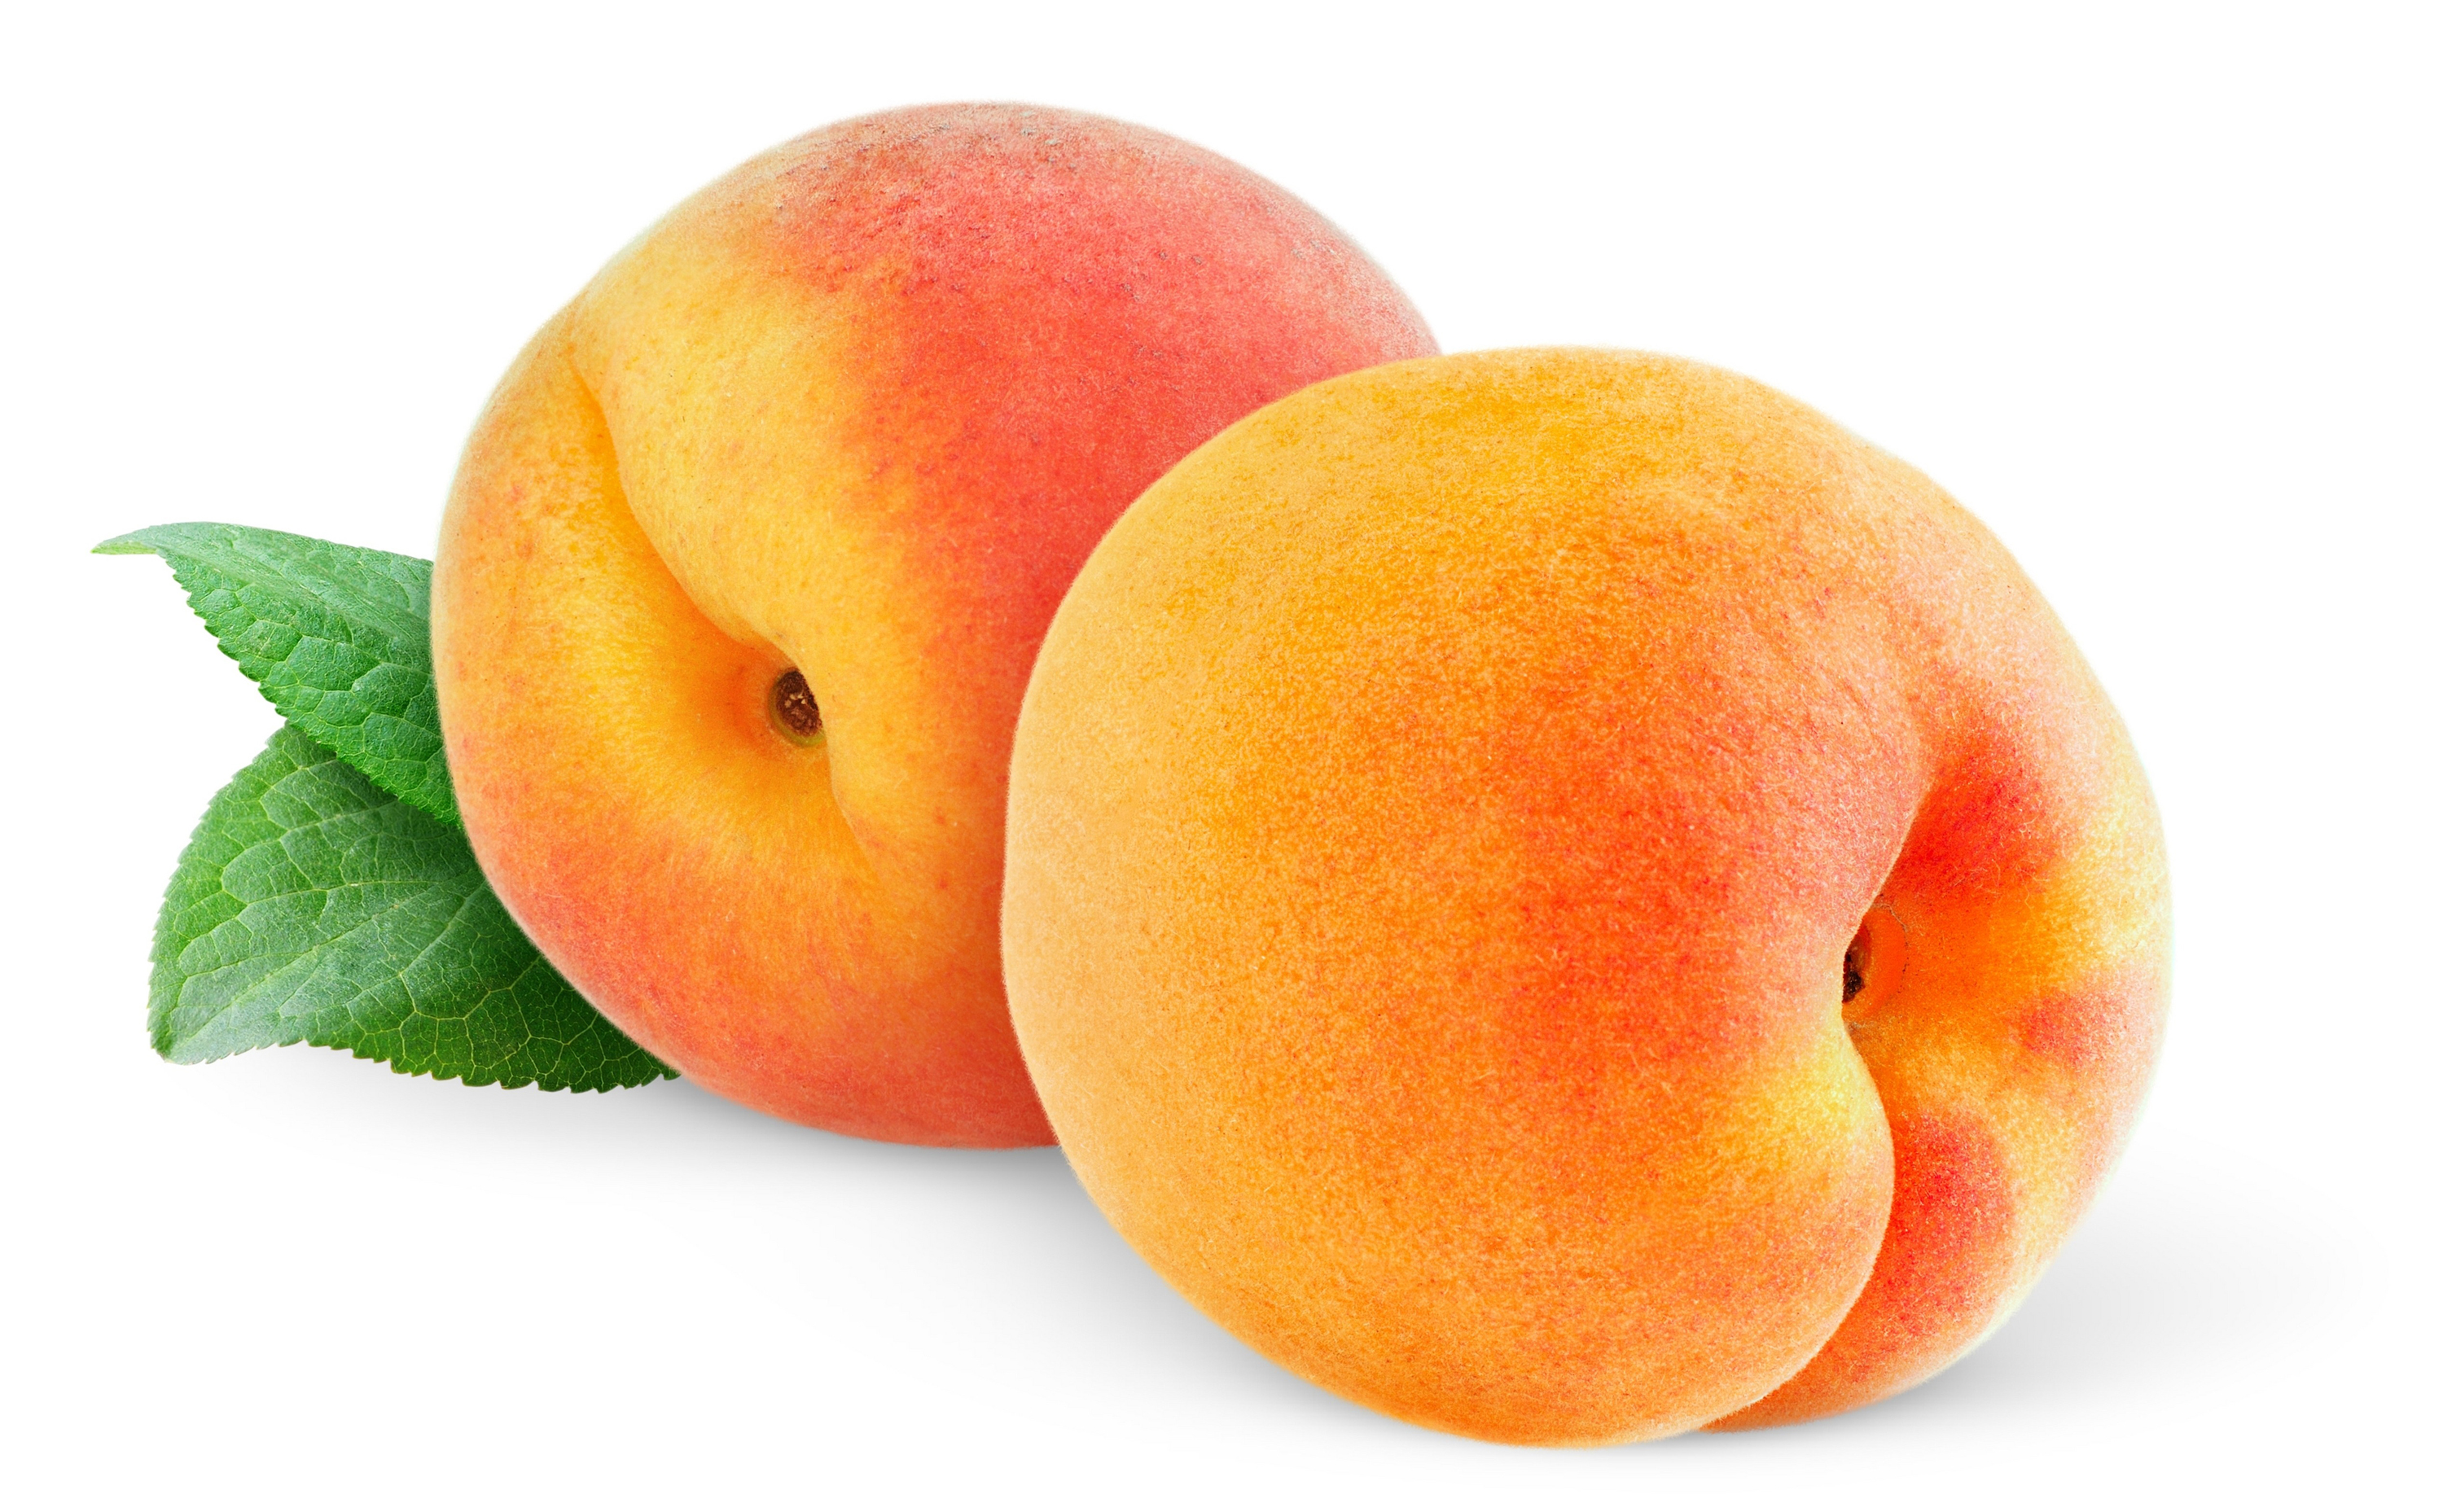
\includegraphics[width=0.8\textwidth]{peachzdfgad.jpg}
  \caption{Delicious peaches although the really new stuff in the paper will be about almonds}
  \label{fig:peach}
\end{figure}



\subsection*{Analysis}
sickle, scythe, bwa-mem, samtools, bcftools...\\
sickle, scythe, bwa-mem, samtools (merge bams), PopBAM, sweepfinder

\section*{Results}

\section*{Discussion}


%\bibliographystyle{apalike} %can use here and not in header
\bibliography{references.bib}

\begin{center}
\begin{longtable}{lllll}
\caption[P. dulcis, P. persica and related species used in analysis.]{P. dulcis, P. persica and related species used in analysis.} \label{my-label} \\
\hline \hline \multicolumn{1}{l}{\textbf{Sample ID}} &
\multicolumn{1}{l}{\textbf{Accession and/or Cultivar}} &
\multicolumn{1}{l}{\textbf{Origin}} &
\multicolumn{1}{l}{\textbf{Source}}  &
\multicolumn{1}{l}{\textbf{Reference}} \\ \hline 
\endfirsthead

\multicolumn{5}{r}{{\bfseries \tablename\ \thetable{} -- continued from previous page}} \\
\hline \multicolumn{1}{l}{\textbf{Sample ID}} &
\multicolumn{1}{l}{\textbf{Accession and/or Cultivar}} &
\multicolumn{1}{l}{\textbf{Origin}} &
\multicolumn{1}{l}{\textbf{Source}} &
\multicolumn{1}{}{\textbf{Reference}} \\ \hline 
\endhead

\hline \multicolumn{5}{r}{{Continued on next page}} \\ \hline
\endfoot

\hline \hline
\endlastfoot

                 \multicolumn{5}{l}{\em{P. dulcis}}  \\
                 %PD01 &DPRU 2578.2 & &NCGR &this study\\ %Almond Board resequencing (BGI)
                 PD02 &‘Tardy Nonpareil’ &USA &UCD &this study\\ %Almond Board resequencing (BGI)
                 PD03 &DPRU 1791.3, BE-1609 & &NCGR &this study\\ %Jastro resequencing (performed at UC Berkeley)
                 PD04 &DPRU 2374.12 & &NCGR &this study\\ %Jastro resequencing (performed at UC Berkeley)
                 PD05 &DPRU 1456.4, Badam & &NCGR &this study\\ %Jastro resequencing (performed at UC Berkeley)
                 PD06 &DPRU 2301, Tuono &Italy &NCGR &this study\\ %Jastro resequencing (performed at UC Berkeley)
                 PD07 &DPRU 1462.2 & &NCGR &this study\\ %Jastro resequencing (performed at UC Berkeley)
                 PD08 &DPRU 1207.2 & &NCGR &this study\\ %Jastro resequencing (performed at UC Berkeley)
                 PD09 &DPRU 2331.9 & &NCGR &this study\\ %Jastro resequencing (performed at UC Berkeley)
                 PD10 &DPRU 0210, Languedoc &France &NCGR &this study\\ %Jastro resequencing (performed at UC Berkeley)
                 PD11 &S3067 & &SRR765861 &\citealt{koepke2013comparative}?\\
                 PD12 &D05-187 & &SRR765850 &\citealt{koepke2013comparative}?\\
                 PD13 &Lauranne & &SRR765838 &\citealt{koepke2013comparative}?\\
                 PD14 &Ramillete & &SRR765679 &\citealt{koepke2013comparative}?\\
                 PD{\color{red}15} &Nonpareil & USA&RosBREED &URL \\
                 \\
                 \multicolumn{5}{l}{\em{P. persica}}  \\ % format italics
                 %PP01 &Lovell & &SRR502985 &\citealt{verde2013high}\\
                 % doubled haploid
                 PP02 &Yumyeong &Korea? &SRR502994 &\citealt{verde2013high}\\
                 PP03 &Shenzhou Mitao&China &\multirow{2}{1cm}{SRR502993, SRR502992} &\citealt{verde2013high}\\
                 %honey peach
                 \\
                 PP04 &Sahua Hong Pantao &China &\multirow{2}{1cm}{SRR502991, SRR502990} &\citealt{verde2013high}\\
                 %flat peach
                 \\
                 PP05 &Quetta & &\multirow{2}{1cm}{SRR502989, SRR502987} &\citealt{verde2013high}\\
                 \\
                 PP06 &Oro A & &SRR502986 &\citealt{verde2013high}\\
                 PP07 &IF7310828 & &\multirow{2}{1cm}{SRR503001, SRR503000} &\citealt{verde2013high}\\
                 \\
                 PP08 &GF305 & &SRR502983 &\citealt{verde2013high}\\
                 PP09 &Contender $\times$ Ambra & &SRR502997 &\citealt{verde2013high}\\
                 % peach x nectarine both P. persica
                 PP10 &Earligold &USA &\multirow{2}{1cm}{SRR502996, SRR502995} &\citealt{verde2013high}\\
                 \\
                 PP11 &Bolero & &SRR501836 &\citealt{verde2013high}\\
                 PP12 &F8,1-42 &USA &SRR068361 &\citealt{ahmad2011whole} \\
                 PP13 &Georgia Belle &USA &SRR068359 &\citealt{ahmad2011whole} \\
                 PP14 &Dr. Davis &USA &SRR068360 &\citealt{ahmad2011whole} \\
                 PP15 &Lovell &USA &UCD &this study\\
                 %(originally a canning variety selected ~1882, curr rootstock) - FPS, ABC
                 %PP &Lovell & &RosBREED &URL \\
                 %originally a canning variety selected ~1882, currently used as rootstock and/or control for disease screening
                 %downloaded?
                 %duplicate cultivar
                 PP{\color{red}X} &DPRU 0589, Early Crawford&USA &RosBREED &URL \\
                 %introduced before 1832
                 PP{\color{red}X} &DPRU 0941, St. John Yellow &USA &RosBREED &URL \\
                 %introduced 1860s
                 PP{\color{red}X} &DPRU 1190, Admiral Dewey&USA &RosBREED &URL \\
                 %aka PI 673525; introduced 1899
                 PP{\color{red}X} &DPRU 2142, Carmen &USA? &RosBREED &URL \\
                 %PI 673586; cultivar original PI 34673 assigned 1912
                 PP{\color{red}X} &DPRU 2179, Slappey &USA &RosBREED &URL \\
                 %aka ‘Slappy’ in GRIN; introduced 1903
                 PP{\color{red}X} &Babcock&USA &RosBREED &URL \\
                 %not yet downloaded
                 %introduced 1897
                 PP{\color{red}X} &Chinese Cling&China &RosBREED &URL \\
                 %introduced 1850; founder several cultivars
                 PP{\color{red}X} &Diamante&Brazil &RosBREED &URL \\
                 %predominant canning cultivar in Brazil per Okie (year & pub TBD)
                 %not yet downloaded
                 PP{\color{red}X} &Dixon&USA? &RosBREED &URL \\
                 %not yet downloaded
                 %PP &Dr. Davis& &RosBREED &URL \\
                 %not downloaded
                 % duplicate cultivar
                 PP{\color{red}X} &Elberta&USA &RosBREED &URL \\
                 %introduced ~1889; OP sdlg of 'Chinese Cling’
                 PP{\color{red}X} &Florida Prince P138&USA? &RosBREED &URL \\
                 %not yet downloaded
                 %PP{\color{red}X} &Georgia Bell&USA &RosBREED &URL \\
                 %(aka ‘Georgia Belle’ and ‘Belle of Georgia’; introduced ~1875; OP sdlg of Chinese Cling)
                 %not downloaded
                 %duplicate cultivar
                 PP{\color{red}X} &JH Hale&USA &RosBREED &URL \\
                 %male sterile; introduced 1912
                 PP{\color{red}X} &Mayflower&USA &RosBREED &URL \\
                 %introduced 1909
                 %not yet downloaded
                 PP{\color{red}X} &Nemaguard &USA &RosBREED &URL \\
                 %rootstock; rumored to have P. davidiana in pedigree
                 PP{\color{red}X} &O’Henry &USA &RosBREED &URL \\
               %CODE FOR APOSTROPHE
                 %plant patent 2.964 1/27/1970; OP sdlg Merrill Bonanza; discovered 1960
                 %not yet downloaded
                 PP{\color{red}X} &Okinawa &? &RosBREED &URL \\
                 PP{\color{red}X} &Oldmixon Free &USA &RosBREED &URL \\
                 % introduced 1832
                 %not yet downloaded
                 PP{\color{red}X} &Rio Oso Gem &? &RosBREED &URL \\
                 %not yet downloaded
                 %some variety history at http://gapeaches.org/about-us/father-of-the-ga-peach-industry/
                 \multicolumn{5}{l}{} \\
                 \multicolumn{5}{l}{Other {\em{Prunus}} species}  \\
                 %Almond Board resequencing (performed at BGI)
                 PF01 &{\em{P. fenzliana}} &? &UCD &this study\\
                 %UCD,ABC
                 PG01 &{\em{P. ferganensis}} &China? &\multirow{2}{1cm}{SRR502999, SRR502998} &\citealt{verde2013high}\\
                 \\
                 PC01 &{\em{P. cerasifera}} DPRU 0579, Myrobalan &? &NCGR &this study\\ \hline
                 %outgroup
                 %NCBI SRA
               %note that the SRR IDs are from NCBI SRA
               %GDR/RosBREED (ftp://ftp.bioinfo.wsu.edu/species/Prunus_persica/RosBREED_Illumina/)

\end{longtable}
\end{center}

\end{document}